\documentclass{beamer}
\usepackage[latin1]{inputenc}
\usepackage{graphicx}
\usetheme{Amsterdam}


\title{ Power line spectrum sensing\\}
\author{Manoj Gulati}
\institute{IIIT-Delhi\\www.iiitd.ac.in}
\date{Jan 15, 2014}
\begin{document}

\begin{frame}
\titlepage
\end{frame}

\begin{frame}
\frametitle{Table of Contents}
\tableofcontents %[currentsection]
\end{frame}

\section{Design Goal} 
\begin{frame}{Design Goal}
Goal: To study effect of voltage fluctuations and building architecture on Conducted EMI.\\
Steps: 
\begin{itemize}
  \item Design a sensor to sense low and high frequency components in power line.
  \item Analyze traces of spectrum with and without test power load.
  \item Analyze traces with EMI filter placed on source side. 
  \ldots
\end{itemize}
\end{frame}

\section{Power line disturbances} 
\begin{frame}{Power line disturbances}
Major cause : Power electronics has become a dominant factor in the deterioration of electromagnetic environment and quality of line power.

EMC: Electromagnetic compatibility is a set of norms laid to restrict amount of low and high frequency disturbances introduced in power line. 
\end{frame}

\section{Categories of EMC} 
\begin{frame}{Categories of EMC}
\begin{figure}[ht!]
%\centering
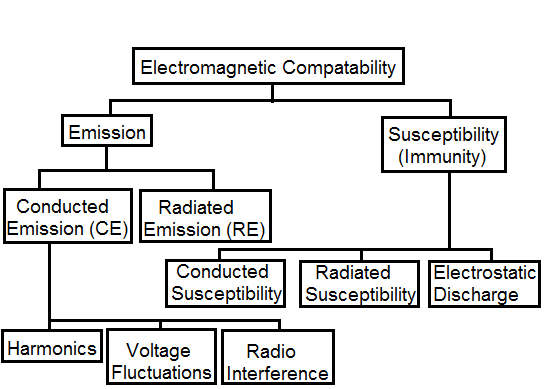
\includegraphics[width=90mm]{EMC_CAT.png}
%\caption{A simple caption}
\label{overflow}
\end{figure}
\end{frame}

\section{Coupling and propagation of Electromagnetic Disturbances} 
\begin{frame}{Coupling and propagation of Electromagnetic Disturbances}
\begin{itemize}
  \item Galvanic Coupling: Disturbing current flows
in a common circuit impedance. Galvanic coupling is reason for conducted emission 
\begin{figure}[ht!]
%\centering
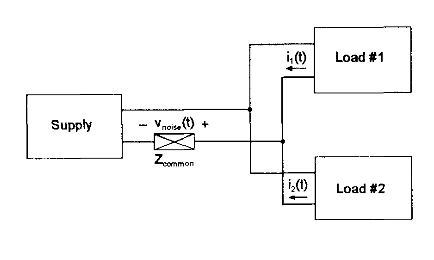
\includegraphics[width=90mm]{FIG_1.png}
%\caption{A simple caption}
\end{figure}
\end{itemize}
\end{frame}

\begin{frame}{Coupling and propagation of Electromagnetic Disturbances}
\begin{itemize}
\item Coupling through electromagnetic near field: Occurs when distance between two conductors is less then $\lambda$/2.
	\begin{itemize}
	\item Capacitive(or electric) Coupling: Disturbing current flows in the capacitance between conductors with ac voltage across them.
	\item Inductive(or magnetic) Coupling: Disturbing current flowing in a loop generates noise voltage across an impedance terminating another loop with mutual inductance to the first loop.
	\end{itemize} 
\end{itemize}
Note: EM Field coupling both near field and far field is reason for radiated emission.
\end{frame}

\begin{frame}{Coupling and propagation of Electromagnetic Disturbances}
\begin{itemize}
\item Capacitive Coupling:
	\begin{figure}[ht!]
	%\centering
	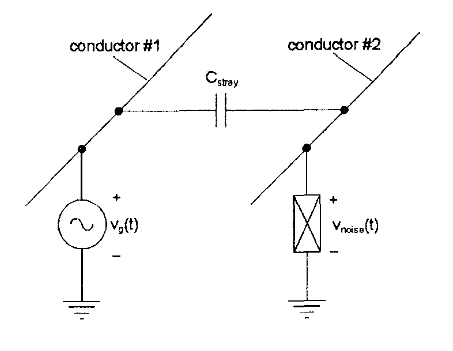
\includegraphics[width=90mm]{FIG_2.png}
	%\caption{A simple caption}
	\end{figure}
\end{itemize}
\end{frame}

\begin{frame}{Coupling and propagation of Electromagnetic Disturbances}
\begin{itemize}
\item Inductive Coupling:
	\begin{figure}[ht!]
	%\centering
	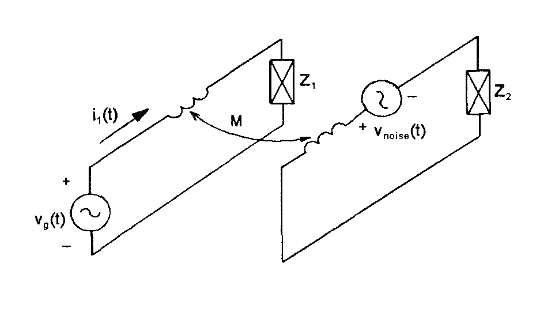
\includegraphics[width=90mm]{FIG_3.png}
	%\caption{A simple caption}
	\end{figure}
\end{itemize}
\end{frame}

\begin{frame}{Coupling and propagation of Electromagnetic Disturbances}
\begin{itemize}
\item Coupling through electromagnetic far field: Occurs when distance between two conductors is much larger then $\lambda$/2.
\end{itemize}
Note: In power electronics coupling through far field is less significant.  
\end{frame}

\begin{frame}{Coupling and propagation of Electromagnetic Disturbances}
\begin{itemize}
\item Coupling through electromagnetic far field:
	\begin{figure}[ht!]
	%\centering
	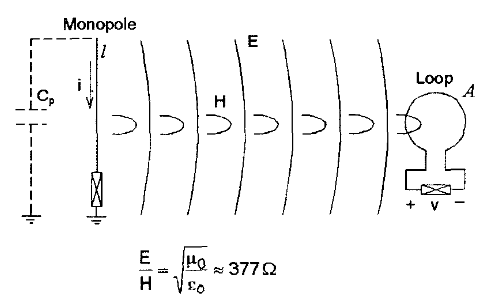
\includegraphics[width=90mm]{FIG_4.png}
	%\caption{A simple caption}
	\end{figure}
\end{itemize}
\end{frame}

\section{Conducted EMI} 
\begin{frame}{Conducted EMI}
Conducted EMI propagates in two ways:
\begin{itemize}
\item Differential mode (or symmetrical): Takes place b/w two conductors, which form a conventional return path. 
\item Common mode (or asymmetrical): Takes place between group of conductors and ground.	
\end{itemize}
\end{frame}

\begin{frame}{Conducted EMI}
	\begin{figure}[ht!]
	%\centering
	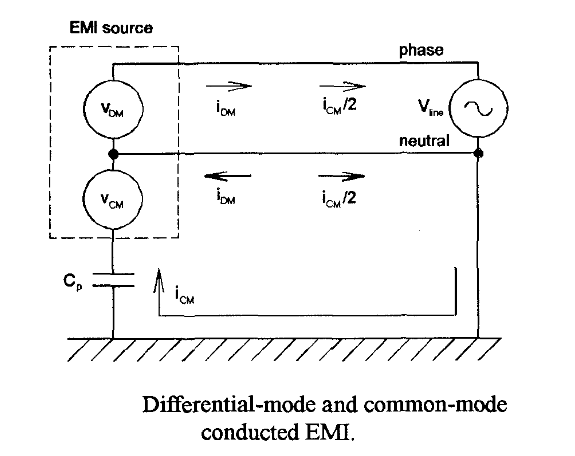
\includegraphics[width=90mm]{FIG_5.png}
	%\caption{A simple caption}
	\end{figure}
\end{frame}

\section{Low frequency disturbances} 
\begin{frame}{Low frequency disturbances}
LF disturbances are harmonic currents and voltages. Harmonic voltages are generated by the voltage drops across distribution impedances while harmonic currents are generated by non-linear loads like diode rectifiers, phase angle controllers etc. 
\end{frame}

\begin{frame}{Low frequency disturbances}
	\begin{figure}[ht!]
	%\centering
	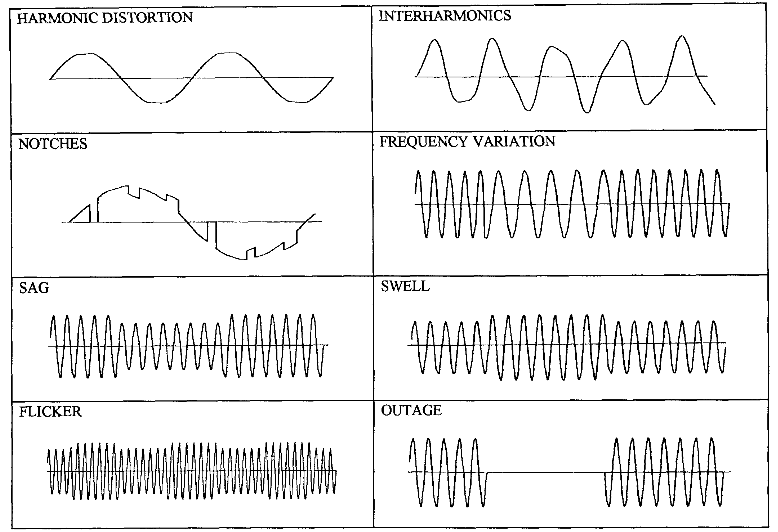
\includegraphics[width=90mm]{FIG_6.png}
	%\caption{A simple caption}
	\end{figure}
\end{frame}

\section{High frequency disturbances} 
\begin{frame}{High frequency disturbances}
HF disturbances are generated by the switching action. Mechanical switches (relays) have high inrush current (capacitive effect) and spark over at breaking contact (inductive effect) and cause wide band emission with continuous spectrum which propagates both with conduction and radiation.
\end{frame}

\begin{frame}{High frequency disturbances}

Another major contributors are periodically switched semi conductor switches (rectifiers, SCRs, BJTs, MOSFETs). They cause differential mode conducted EMI through basic power conversion process and common mode conducted EMI through capacitive or inductive coupling.\\

HF(\textgreater10MHz)EMI spectrum also propagates through radiation.  
\end{frame}

\section{References} 
\begin{frame}{References}
\begin{itemize}
\item Power Electronics and Electromagnetic Compatibility 
\item Electromagnetic Interference (EMI) in 
Power Supplies
\item ElectriSense: Single-Point Sensing Using EMI for Electrical Event Detection and Classification in the Home
\item \href{http://www.electrical-installation.org/enwiki/EMC_-_Coupling_mechanisms_and_counter-measures}{Coupling mechanisms (Click to access web link)}
\end{itemize}
\end{frame}

\end{document}